\documentclass{slides}

\lstset{language=C++}
\usepackage{array}
\usepackage{xspace}

\begin{document}
\newcommand{\ie}{\textit{i.\thinspace e.}\xspace}
\newcommand{\eg}{\textit{e.\thinspace g.}\xspace}

\graphicspath{{figures/}}

\title[Programming in C++: Outline]{\Large Programming in C++: Outline}

\author[A. Arnold and O. Lenz]{Axel Arnold \and Olaf Lenz} 
\institute{Institut für Computerphysik\\Universit\"at Stuttgart}
\date{February 18-22, 2013}

\setbeamertemplate{footline}{}
\begin{frame}
  \titlepage
\end {frame}
\setbeamertemplate{footline}[icp]

\begin{frame}
  \frametitle{General Information}
  \begin{itemize}
  \item „Fachübergreifende Schlüsselqualifikation, Kompetenzbereich 1“
  \item 3 LP
  \item Requirement: Basic knowledge of programming\\ (C, FORTRAN \emph{or} Python)
  \item Lectures in the morning (9:15 - 12:30)
  \item Exercises in the afternoon (14:00 - 17:00)
    \begin{itemize}
    \item Some small exercises
    \item One project: „Finstere Flure“
    \item Possibly a tournament on Friday
    \end{itemize}
  \item We are open to suggestions
  \end{itemize}
\end{frame}

\begin{frame}
  \frametitle{Contents}
  \begin{itemize}
  \item Day 1
    \begin{itemize}
    \item The C in C++ I
    \item Object-oriented design
    \end{itemize}
  \item Day 2
    \begin{itemize}
    \item The C in C++ II
    \item OO concepts in C++
    \end{itemize}
  \item Day 3
    \begin{itemize}
    \item Objects and encapsulation in C++
    \item Inheritance and polymorphism in C++
    \end{itemize}
    \item Day 4
      \begin{itemize}
      \item Exceptions and namespaces
      \item Data type conversions in C++
      \end{itemize}
    \item Day 5
      \begin{itemize}
      \item Templates and STL
      \item Software development models
      \end{itemize}
  \end{itemize}
\end{frame}

\begin{frame}
  \frametitle{Recommended Literature}
  \begin{itemize}
  \item Best online ressource: \url{http://www.cplusplus.com}
  \item \textit{Thinking in C++: Introduction to Standard C++} by
    Bruce Eckel (Prentice Hall; 2nd edition; 2000)
    \begin{itemize}
    \item Free online book
    \item Good to learn about the ideas
    \item Meanwhile somewhat outdated
    \item ``TICPP''
    \item \dots what this course is based on
    \end{itemize}
  \item \textit{Thinking in C++: Practical Programming} by Bruce Eckel
    and Chuck Allison (Prentice Hall; 1st edition, 2003)
  \item \textit{The C++ Programming Language} by Bjarne Stroustrup
    (Addison-Wesley Professional; 4 edition, 2013)
    \begin{itemize}
    \item The reference for all things C++
    \item Not yet out
    \item Includes new \textit{C++11} standard
    \item Not very good to \emph{learn} the language
    \end{itemize}
  \end{itemize}
\end{frame}

\begin{frame}
  \frametitle{History of C}
  \begin{columns}[c,onlytextwidth]
    \column{0.6\textwidth}
    \begin{tabular}{r<{:}p{0.8\textwidth}}
      1969 -- 73 & Developed by D. M. Ritchie (based on ``B'')\\
      1978 & ``\emph{The C Programming Language}'' by Kernighan und Ritchie (``K\&R-C'')\\
      1989 & Standard ANSI C89 = ISO C90\\
      1999 & Standard ISO C99\\
      2011 & Standard ISO C11
    \end{tabular}

    \column{0.3\textwidth}
    \centering
    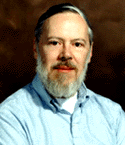
\includegraphics[height=0.25\textheight]{ritchie}\\
    {\small D. M. Ritchie\\1941 -- 2011}
  \end{columns}
  \vspace{0.5em}

  \begin{itemize}
  \item ``Procedural'' language
  \item Nowadays used mainly for system and embedded programming
    \begin{itemize}
    \item Operating systems (\eg Unix, Windows)
    \item Other programming languages (\eg Python)
    \item \dots and in physics (only the young ones, the old ones use FORTRAN)
    \end{itemize}
  \item In this course, we will not distinguish between C and C++
  \end{itemize}
\end{frame}

\begin{frame}
  \frametitle{History of Object-Oriented Programming and C++}
  \begin{columns}[c,onlytextwidth]
    \column{0.5\textwidth}
    \begin{tabular}{r<{:}p{0.9\textwidth}}
      1967 & \textit{Simula 67}: first OO language by O. Dahl and K. Nygaard\\
      1979 & B. Stroustrup develops ``C with classes'' based on Simula 67\\
      1983 & Language is renamed to \textbf{C++}\\
      1985 & ``\emph{The C++ Programming Language}'' by Stroustrup\\
      1998 & Standard ISO C++98\\
      2011 & Standard ISO C++11
    \end{tabular}

    \column{0.5\textwidth}
    \centering
    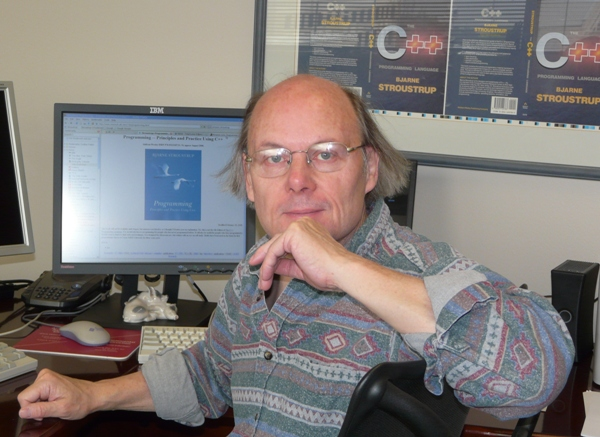
\includegraphics[height=0.25\textheight]{stroustrup}\\
    {\small B. Stroustrup, *1950}
  \end{columns}

  \vspace{0.5em}
  \begin{itemize}
  \item OOP was seen as a possible solution to the ``software crisis''
  \item Most languages nowadays are object-oriented (\eg Java, C\#, Python, \dots)
  \item C++: C with Objects
  \item C++11-standard is explicitly marked
  \end{itemize}

\end{frame}

\begin{frame}
  \frametitle{Features of C++}
  C++ \dots
  \begin{description}
  \item[\dots is compatible with C.] \emph{Was} important, now a problem.
  \item[\dots is an imperative, procedural programming language.]
  \item[\dots is an object-oriented programming language.]
  \item[\dots is a compiled language.] The code is translated (\textit{compiled}) into machine code
    by a \textit{compiler}.
  \item[\dots can be used for low-level programming.] Hardware can be programmed pretty directly.
  \item[\dots is (pretty much) portable.] A C++ compiler exists for virtually any platform. However,
    the dialects vary.
  \item[\dots has libraries for anything.] 
  \item[\dots is used for almost anything.] Many application programs are implemented in C++.
  \end{description}
\end{frame}

\begin{frame}
  \vfill
  \centering
  \Huge Let's go \dots
  \vfill
\end{frame}

\end{document}
